% AML期刊elsarticle模板规范
\documentclass[3p]{elsarticle}
% Use the option review to obtain double line spacing
% \documentclass[final,1p,times,twocolumn,authoryear]{elsarticle}
% 必要宏包
\usepackage{amssymb}
\usepackage{amsmath}
\usepackage{graphicx}
\usepackage{multirow}
\usepackage{paralist}
\usepackage{color}
\usepackage{float}
\usepackage{nicematrix}
\usepackage{tikz}
\usetikzlibrary{matrix,decorations.pathreplacing}
\usepackage{arydshln}%虚线
\usepackage{algorithm} % 算法
\usepackage{algmatlab}

% elsarticle依赖包
\usepackage{natbib} % 引文处理
\usepackage{geometry} % 页边距设置
% \usepackage{fleqn} % 左对齐公式
\usepackage{graphicx} % 插入图形
% \usepackage{txfonts} % 如果文档要用Times字体和与之兼容的数学字体进行排版
% \usepackage{hyperref} % 超链接
% \usepackage{endfloat} % 如果要将浮动体放在PDF末尾。

% 其他数学环境
\newtheorem{theorem}{Theorem}[section]
\newtheorem{definition}[theorem]{Definition}
\newtheorem{lemma}[theorem]{Lemma}
\newtheorem{corollary}[theorem]{Corollary}
\newtheorem{proposition}[theorem]{Proposition}
\newtheorem{example}[theorem]{Example}
\newtheorem{remark}[theorem]{Remark}
\newenvironment{proof}{\noindent {\bf Proof.\ }}{\vspace{2ex}}

\numberwithin{equation}{section}

\begin{document}

%-------------------- FRONTMATTER --------------------
\begin{frontmatter}

% 标题
\title{An Algorithm for QR Decomposition of Split Quaternion Matrices}

% 作者与机构
\author[inst1]{Qianqian Liu}
\author[inst1]{Xin Liu\corref{cor1}}
\ead{xiliu@must.edu.mo}
\author[inst1]{Jianhai Lin\fnref{fn1}}
\author[inst2]{Yang Zhang}

\cortext[cor1]{Corresponding author}
\tnotetext[fund]{This research is supported by Macao Science and Technology Development Fund (No. 0013/2021/ITP), the grants from the National Natural Science Foundation of China (12371023, 12271338), and the Natural Sciences and Engineering Research Council of Canada (NSERC) (RGPIN 2020-06746), The joint research and Development fund of Wuyi University, Hong Kong and Macao (2019WGALH20), Macau University of Science and Technology Faculty Research Grants (FRG-22-073-FIE).}

\address[inst1]{Faculty of Innovation Engineering, Macau University of Science and Technology, Avenida Wai Long, TaiPa, Macau, 999078, P. R. China}
\address[inst2]{Department of Mathematics, University of Manitoba, Winnipeg, MB, R3T 2N2, Canada}
\fntext[fn1]{The author designed and implemented Algorithms \ref{alg:Permutation}, \ref{alg:Permutation Optimization}, and \ref{alg:QR}.}

% 摘要
\begin{abstract}
Split quaternions contain zero divisors, thus it is not a Euclidean distance space. Therefore, the traditional QR decomposition based on Givens rotations and Householder reflection transformations is difficult to implement. To overcome this difficulty and to address the non-commutativity of split quaternion multiplication, we will utilize the real representation $A^\sigma$ of the split quaternion matrix $A$.  By leveraging the proposed decomposition $A^\sigma = \hat{Q}R_4$  ($\hat{Q}$ is an orthogonal matrix, and $R_4 = \begin{bmatrix} R_{11} & R_{12} \\ R_{21} & R_{22} \end{bmatrix}$, with $R_{11}, R_{12}, R_{21}, R_{22}$ being upper triangular), the QR decomposition of the split quaternion matrix was successfully constructed using its real representations. To verify its effectiveness, the proposed algorithm was used for QR decomposition and solving a matrix equation, and the experimental results demonstrate its high efficiency in CPU time and accuracy.
\end{abstract}

% 关键词
\begin{keyword}
Split quaternion matrix \sep QR decomposition \sep Permutation matrix \sep Upper triangular matrix
\end{keyword}

\end{frontmatter}

%-------------------- 正文主体 --------------------

\section{Introduction}
In 1849, James Cockle \cite{Cockle1849} introduced the concept of split quaternion algebra over the real numbber field $\mathbb{R}$,   which can be described by the following rules:
\begin{equation*}
    \small
    \mathbb{H}_s = \left\{ a_0 + a_1 i + a_2 j + a_3 k \ \bigg| i^2 = -1,\ j^2 = k^2 = 1, \ ijk = 1, \ a_0, a_1, a_2, a_3 \in \mathbb{R} \right\} 
\end{equation*} 
$\mathbb{H}_s$ is a four dimensional commutative algebra over $\mathbb{R}$ and contains zero divisors. 
Split quaternion matrices have found applications in quantum mechanics, electromagnetism and signal processing (see, e.g.,\cite{Gog2022},\cite{Hasebe2010},\cite{Le2022},\cite{Z2022},\cite{Wang2023}). In the past decades, many researches  have been done in studying the algebraic properties of split quaternions (see, e.g., \cite{Abłamowicz2020},\cite{Yasemin2012},\cite{TJiang2015}-\cite{TJiang2018},\cite{Zhuo2020}-\cite{Xin2019},\cite{mma},\cite{wang},\cite{Wang2021}-\cite{Zhang2015}). For instance, \cite{Jiang2018}-\cite{TJiang2018} respectively solved the eigenvalue problems and the solutions to the Schrödinger equation; \cite{Xin2019} derived a new real representation of split quaternion matrices to explain the consistency of two types of split quaternion matrix equations \(AX^* - XB = CY + D\) and \(X - AX^*B = CY + D\); \cite{wang} solved the classical system of matrix equations; \cite{Wang2021} proposed a fast algorithm based on LDU decomposition;  \cite{Gang2024}  proposed the SVD decomposition theory and an efficient algorithm for decomposing quaternion matrices. However, the existing research has yet to fully address the theoretical development and algorithmic implementation of QR decomposition for split quaternion matrices.

To address the above problem, we constructively prove the existence of QR decomposition for split quaternion matrices, and we propose a novel and efficient algorithm for computing this QR decomposition.  To validate the efficiency  of our algorithm, we provide the experimental results in terms of speed and accuracy.

\section{Preliminaries}
For any split quaternion matrix ${A}=A_{0}+A_{1}i + A_{2}j + A_{3}k \in\mathbb{H}_{s}^{m\times n}$, where $A_{i}\in\mathbb{R}^{m\times n}, i\in\{0,1,2,3\}$, its transpose, conjugate, conjugate transpose, i-conjugate, and i-conjugate transpose are  denoted by 
 ${A}^T = A_0^T + A_1^Ti + A_2^Tj + A_3^Tk,\bar{{A}} = A_0 - A_1i - A_2j - A_3k, {A}^* = A_0^T - A_1^Ti - A_2^Tj - A_3^Tk,$ and $\tilde{{A}} = A_0 - A_1i + A_2j + A_3k,{A}^H = A_0^T - A_1^Ti + A_2^Tj + A_3^Tk$, respectively.

The real representation matrix of a split quaternion matrix is presented as \cite{Gang2024}:
\begin{equation}\label{eq:2.1}
{A}^\sigma = \begin{bmatrix} A_0 + A_2 & -A_1 + A_3 \\ A_1 + A_3 & A_0 - A_2 \end{bmatrix} \in \mathbb{R}^{2m \times 2n},
\end{equation}
which has the properties
\begin{equation}\label{eq:2.2}
\begin{aligned}
    (A + B)^\sigma = A^\sigma + B^\sigma, \quad (AC)^\sigma = A^\sigma C^\sigma, 
    (a A)^\sigma = a A^\sigma, \quad (tA^H)^\sigma = (A^\sigma)^H
\end{aligned}
\end{equation}
where $A, B \in \mathbb{H}_s^{m \times n}$, $C \in \mathbb{H}_s^{n \times p}$, $a \in \mathbb{R}$. 

Conversely, for any real matrix $B = \begin{bmatrix} B_{11} & B_{12} \\ B_{21} & B_{22} \end{bmatrix} \in \mathbb{R}^{2m \times 2n}$, $B_{ts} \in \mathbb{R}^{m \times n}$, $t, s = 1, 2$, one can construct a corresponding split quaternion matrix $A$ as follows \cite{TJiang2015}:
\begin{equation}\label{eq:2.3}
    \begin{aligned}
    A = \frac{B_{11} + B_{22}}{2} + \frac{B_{21} - B_{12}}{2}i 
        + \frac{B_{11} - B_{22}}{2}j + \frac{B_{21} + B_{12}}{2}k.
    \end{aligned}
    \end{equation}
From equation \eqref{eq:2.1}, we have ${A}^\sigma = B$. 
That is,  $\sigma$ provides an one-to-one corresponding between $\mathbb{H}_s^{m\times n}$ and $\mathbb{R}^{2m \times 2n}$ \cite{Gang2024}.

Furthermore,  $A$ is called unitary if $AA^H = A^H A = I$. We can verify that $A$ is unitary if and only if  $A^\sigma$ is  orthogonal (\cite{TJiang2018}).
 The Frobenius norm of $A$ is defined as: 
 \begin{align*}
     \| A \|_F \equiv \frac{1}{\sqrt{2}} \| A^\sigma \|_F = \sqrt{\| A_0 \|_F^2 + \| A_1 \|_F^2 + \| A_2 \|_F^2 + \| A_3 \|_F^2}.
\end{align*}
  When $U, V$ are unitary, $U^\sigma$ and $V^\sigma$ are orthogonal, which will not change the Frobenius norm  of $A^\sigma$. Hence
\begin{align*}
\|UAV\|_F = \frac{1}{\sqrt{2}} \|(UAV)^\sigma\|_F 
= \frac{1}{\sqrt{2}} \|U^\sigma A^\sigma V^\sigma\|_F 
= \frac{1}{\sqrt{2}} \|A^\sigma\|_F 
= \|A\|_F.
\end{align*}

\section{QR Decomposition of Split Quaternion matrix}
In this section, we discuss the QR decomposition for split quaternion matrices through construction, and develop an efficient algorithm.

Let $A \in \mathbb{H}^{m \times n}$, we use the following two steps to construct its QR decomposition.  

\textbf{Step 1:} Perform the decomposition of $A^\sigma \in \mathbb{R}^{2m \times 2n}$ as 
\begin{equation}\label{splitqr}
A^\sigma = \widetilde{Q} R_4,
\end{equation} 
where $\widetilde{Q} \in \mathbb{R}^{2m\times 2m}$ is an orthogonal matrix, and $R_4  $ is a block matrix given by:
\begin{equation}\label{r4}
R_4 = \begin{bmatrix}
    R_{11} & R_{12} \\
    R_{21} & R_{22}
\end{bmatrix} \in \mathbb{R}^{2m \times 2n},
\end{equation}
and $R_{11}, R_{12},R_{21},R_{22}$ are all upper triangular matrices of size $m \times n$.

To achieve the special decomposition \eqref{splitqr},  we will first figure out how to transform an upper triangular matrix $R$ into $R_4$ through permutation transformations, as depicted in Figure below. It is the key to realize the special decomposition \eqref{splitqr}
\begin{figure}[htbp]
    % \begin{minipage}[htbp]{0.45\textwidth}
        \centering
        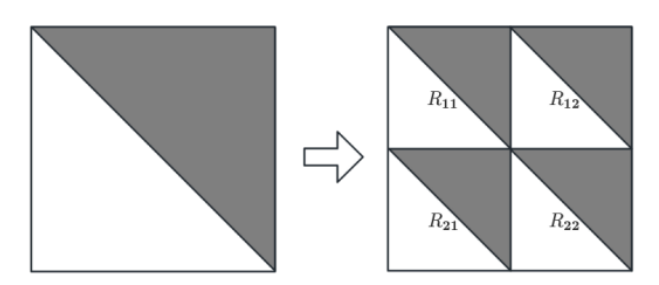
\includegraphics[width=0.45\textwidth,keepaspectratio=true]{Upper triangular.png} % Replace with actual file name
         % \caption{Transformation of a $2n \times 2n$ upper triangular matrix.}
         \label{fig:Upper triangular}
    % \end{minipage}
\end{figure}

To better understand the procedure, we will choose the matrix 
\[R= \begin{bmatrix}
\begin{array}{cc:cc:cc}
 r_{11} & r_{12} & r_{13} & r_{14} & r_{15} & r_{16}\\
 0 & r_{22} & r_{23} & r_{24} & r_{25} & r_{26}\\
 \cdashline{1-6}
 0      & 0      & r_{33} & r_{34} & r_{35} & r_{36}\\
 0      & 0      & 0 & r_{44} & r_{45} & r_{46}\\
 \cdashline{1-6}
 0      & 0      & 0      & 0      & r_{55} & r_{56}\\
 0      & 0      & 0      & 0      & 0 & r_{66}\\
\end{array}
\end{bmatrix}
\]
to demonstrate. 

We  perform the following swaps in matrix $R$:
\begin{align*}
R
& \xrightarrow{r_{2} \leftrightarrow r_{5}}
\begin{bmatrix}
% \begin{array}{cc:cc:cc}
 r_{11} & r_{12} & r_{13} & r_{14} & r_{15} & r_{16}\\
 0      & 0      & 0      & 0      & r_{55} & r_{56}\\
 0      & 0      & r_{33} & r_{34} & r_{35} & r_{36}\\
 \cdashline{1-6}
 0      & 0      & 0 & r_{44} & r_{45} & r_{46}\\
 0 & r_{22} & r_{23} & r_{24} & r_{25} & r_{26}\\
 0      & 0      & 0      & 0      & 0 & r_{66}\\
% \end{array}
\end{bmatrix}
\xrightarrow{r_{2} \leftrightarrow r_{3}}
\begin{bmatrix}
% \begin{array}{cc:cc:cc}
 r_{11} & r_{12} & r_{13} & r_{14} & r_{15} & r_{16}\\
 0      & 0      & r_{33} & r_{34} & r_{35} & r_{36}\\
 0      & 0      & 0      & 0      & r_{55} & r_{56}\\
 \cdashline{1-6}
 0      & 0      & 0 & r_{44} & r_{45} & r_{46}\\
 0 & r_{22} & r_{23} & r_{24} & r_{25} & r_{26}\\
 0      & 0      & 0      & 0      & 0 & r_{66}\\
% \end{array}
\end{bmatrix} \\
& \xrightarrow{r_{4} \leftrightarrow r_{5}}
\begin{bmatrix}
% \begin{array}{cc:cc:cc}
 r_{11} & r_{12} & r_{13} & r_{14} & r_{15} & r_{16}\\
 0      & 0      & r_{33} & r_{34} & r_{35} & r_{36}\\
 0      & 0      & 0      & 0      & r_{55} & r_{56}\\
 \cdashline{1-6}
 0 & r_{22} & r_{23} & r_{24} & r_{25} & r_{26}\\
 0      & 0      & 0 & r_{44} & r_{45} & r_{46}\\
 0      & 0      & 0      & 0      & 0 & r_{66}\\
% \end{array}
\end{bmatrix}
\xrightarrow{c_{2} \leftrightarrow c_{5}}
\begin{bmatrix}
\begin{array}{ccc:ccc}
 r_{11} & r_{15} & r_{13} & r_{14}  & r_{12} & r_{16}\\
 0      & r_{35} & r_{33} & r_{34}  & 0      & r_{36}\\
 0      & r_{55} & 0      & 0       & 0      & r_{56}\\
 \cdashline{1-6}
 0      & r_{25} & r_{23} & r_{24}  & r_{22} & r_{26}\\
 0      & r_{45} & 0      & r_{44}  & 0      & r_{46}\\
 0      & 0      & 0      & 0       & 0      & r_{66}\\
\end{array}
\end{bmatrix} \\
& \xrightarrow{c_{2} \leftrightarrow c_{3}}
\begin{bmatrix}
\begin{array}{ccc:ccc}
 r_{11} & r_{13} & r_{15} & r_{14}  & r_{12} & r_{16}\\
 0      & r_{33} & r_{35} & r_{34}  & 0      & r_{36}\\
 0      & 0      & r_{55} & 0       & 0      & r_{56}\\
 \cdashline{1-6}
 0      & r_{23} & r_{25} & r_{24}  & r_{22} & r_{26}\\
 0      & 0      & r_{45} & r_{44}  & 0      & r_{46}\\
 0      & 0      & 0      & 0       & 0      & r_{66}\\
\end{array}
\end{bmatrix}
\xrightarrow{c_{4} \leftrightarrow c_{5}}
\begin{bmatrix}
\begin{array}{ccc:ccc}
 r_{11} & r_{13} & r_{15} & r_{12} & r_{14} & r_{16}\\
 0      & r_{33} & r_{35} & 0      & r_{34} & r_{36}\\
 0      & 0      & r_{55} & 0      & 0      & r_{56}\\
 \cdashline{1-6}
0 & r_{23} & r_{25} & r_{22} & r_{24} & r_{26}\\
 0      & 0 & r_{45} & 0      & r_{44} & r_{46}\\
 0      & 0      & 0 & 0      & 0      & r_{66}\\
\end{array}
\end{bmatrix} \\
&=\begin{bmatrix}
    R_{11} & R_{12}\\R_{21} & R_{22}
\end{bmatrix} = R_4
\end{align*}


% Perform the following row exchanges, $r_{2} \leftrightarrow r_{5}$, then $r_{2} \leftrightarrow r_{3}$, and $r_{4} \leftrightarrow r_{5}$. Perform the same exchanges for the columns, $c_{2} \leftrightarrow c_{5}$, then $c_{2} \leftrightarrow c_{3}$, and $c_{4} \leftrightarrow c_{5}$. We can obtain the following \\
% We  perform the following swaps in matrix $R$: {\color{red} Replace the odd rows (1, 3, 5) sequentially with the first three rows. Replace the even rows (2, 4, 6) sequentially with the last three rows. Replace the odd columns (1, 3, 5) sequentially with the first three columns. Replace the even columns (2, 4, 6) sequentially with the last three columns. ????} We can obtain the following  resulting matrix:

% \[R_4 = \begin{bmatrix}
% \begin{array}{ccc:ccc}
%  r_{11} & r_{13} & r_{15} & r_{12} & r_{14} & r_{16}\\
%  0      & r_{33} & r_{35} & 0      & r_{34} & r_{36}\\
%  0      & 0      & r_{55} & 0      & 0      & r_{56}\\
%  \cdashline{1-6}
% 0 & r_{23} & r_{25} & r_{22} & r_{24} & r_{26}\\
%  0      & 0 & r_{45} & 0      & r_{44} & r_{46}\\
%  0      & 0      & 0 & 0      & 0      & r_{66}\\
% \end{array}
% \end{bmatrix}=\begin{bmatrix}
%     R_{11} & R_{12}\\R_{21} & R_{22}
% \end{bmatrix}.
% \]
  The above process  applies to any upper triangular matrices $R$ with even orders $2m \times 2n$. Theoretically, the relationship between $R$ and $R_4$ is as follows:
\begin{equation}\label{eq:Rn}
    P_{m} R P_{n}^T = \begin{bmatrix} R_{11} & R_{12}\\R_{21}& R_{22}\end{bmatrix}.
\end{equation}
To obtain the matrix $P_k, k\in \{m,n\}$ for $R \in \mathbb{R}^{2m \times 2n}$, we established Algorithm \ref{alg:Permutation}. When the input is $A=I_{2k \times 2k}$ and $flag=0$, we can obtain the permutation matrix $P_k$:

\begin{equation}\label{p}
    P_k = \begin{bmatrix} 
            1 & 0 & 0 & 0 & \cdots & 0 & 0\\ 
            0 & 0 & 1 & 0 & \cdots & 0 & 0\\ 
            \vdots & \vdots & \vdots & \vdots &  & \vdots & \vdots\\ 
            0 & 0 & 0 & 0 & \cdots & 1 & 0 \\
            0 & 1 & 0 & 0 & \cdots & 0 & 0\\ 
            0 & 0 & 0 & 1 & \cdots & 0 & 0\\ 
            \vdots & \vdots & \vdots & \vdots &  & \vdots & \vdots\\ 
            0 & 0 & 0 & 0 &\cdots & 0 & 1 
        \end{bmatrix}_{2k \times 2k}
\end{equation}
{\color{red} We can see that $P_k$ is a permutation matrix. By proposing this $P_k$, we successfully transform an even-order upper triangular $R$ matrix into an $R_4$ matrix \eqref{r4}.}


\begin{algorithm}[htbp]
    \caption{Matrix Permutation Recursive Algorithm} \label{alg:Permutation}
    \begin{algorithmic}
    \Function{Permutation}{$A,\text{flag}$}
        \State \% \textbf{Input:} $A \in \mathbb{R}^{s \times 2n}$, where flag=0 represents the first submatrix 
        \State \% \qquad\quad\ and flag=1 represents the second submatrix.
        \State \% \textbf{Output:} $B \in \mathbb{R}^{s \times 2n}$.
        \State \% \textbf{Step 1} Recursive stop condition:
        \If{$s=2$} \State $B=A$; \Return \ $B$;\End
        \State \% \textbf{Step 2} Initialization:
        \State $s2 = \text{floor}((s+1)/2)$;
        \State $s3 = \text{floor}(s2/2)$;
        \State \% \textbf{Step 3} Add zero rows:
        \If{$\text{mod}(s, 2)=1$}
            \If{flag=1}
                \State $A = [\text{zeros}(1, \text{size}(A, 2)); A]$;
            \Else
                \State $A = [A; \text{zeros}(1, \text{size}(A, 2))]$;
            \End
        \End
        \State \% \textbf{Step 4} Perform swapping:
        \For{$i=1:s3$}
            \If{$\text{mod}(s2, 2)=0$}
                \State $A= \text{swap}(A,2*i,s2+2*(i-1)+1)$;
            \Else
                \State $A= \text{swap}(A,2*i,s2+2*(i-1)+2)$;
            \End
        \End
        \State \% \textbf{Step 5} Recursive execution:
        \State $A(1:s2, :) = \text{Permutation}(A(1:s2, :), 0)$;
        \State $A(s2+1:\text{end}, :) = \text{Permutation}(A(s2+1:\text{end}, :), 1)$;
        \State \% \textbf{Step 6} Remove zero rows:
        \If{$\text{mod}(s, 2)=1$}
            \If{flag=1}
                \State $B = A(2:\text{end}, :)$;
            \Else
                \State $B = A(1:\text{end}-1, :)$;
            \End
        \Else
            \State $B=A$;
        \End
    \End 
    \end{algorithmic}
\end{algorithm}

% \begin{algorithm}[htbp]
%     \caption{Matrix Permutation Algorithm} \label{alg:Permutation}
%     \textbf{Function:} $B=\text{Permutation}(A,\text{flag})$\\	
%     \textbf{Input:}  $ A \in \mathbb{R}^{k \times 2n}$, where flag=0 represents the first submatrix and flag=1 represents the second submatrix.\\
%     \textbf{Output:} $B \in \mathbb{R}^{k \times 2n}$ .
% \begin{itemize}
%     \item[\textbf{Step 1}]\text{ Recursive stop condition:}\\
%         \text{if} $k=2$ \quad return $B=A$;
%     \item[\textbf{Step 2}] Initialization:\\
%         $k2 = \text{floor}((k+1)/2)$;\\
%         $k3 = \text{floor}(k2/2)$;
%     \item[\textbf{Step 3}] Add zero rows:\\
%         if $\text{mod}(k, 2)=1$ \\
%         \quad \quad if flag=1 \ $A = [\text{zeros}(1, \text{size}(A, 2)); A]$;\\
%         else  $A = [A; \text{zeros}(1, \text{size}(A, 2))]$;
%     \item[\textbf{Step 4}] Perform swapping:\\
%        for $i=1:k3$\\
%        if $\text{mod}(k2, 2)=0$ \quad
%         $A= \text{swap}(A,2*i,k2+2*(i-1)+1)$;\\
%        else
%         $A= \text{swap}(A,2*i,k2+2*(i-1)+2)$;
%     \item[\textbf{Step 5}] Recursive execution:\\
%        $A(1:k2, :) = \text{Permutation}(A(1:k2, :), 0)$;\\
%        $A(k2+1:\text{end}, :) = \text{Permutation}(A(k2+1:\text{end}, :), 1)$;
%     \item[\textbf{Step 6}] Remove zero rows: \\
%        if $\text{mod}(k, 2)=1$ \\
%        if flag=1 \quad $B = A(2:\text{end}, :)$;\\
%        else $B = A(1:\text{end}-1, :)$;
%     \item[\textbf{Step 7}] return $B=A$;
% \end{itemize}
% \end{algorithm}
After completing the above steps, we can now proceed to implement the decomposition \eqref{splitqr}.
First, perform the QR decomposition to the real matrix $P_m^TA^\sigma P_{n}$:
$$P_m^TA^\sigma P_n = \widehat{Q}\widehat{R}.$$
According to \eqref{eq:Rn}, we have
$$
P_m^TA^\sigma P_n = \widehat{Q}\widehat{R} = \widehat{Q}(P_m^TR_4P_n).
$$
Multiplying both sides of the equation by $P_m$ on the left and $P_n^T$ on the right yields
$$
A^\sigma=P_m\widehat{Q}P_m^T R_4.
$$
Since $P_m$ is a permutation matrix, it is also an orthogonal matrix. Thus, the product of matrices, $P_m\widehat{Q}P_m^T$, is also an orthogonal matrix. Then we get our required special decomposition $A^\sigma=\widehat{Q}R_4,$ where $\widetilde{Q}=P_m\widehat{Q}P_m^T$ is orthogonal, and $R_4$ is in the form of \eqref{r4}.

% \begin{algorithm}[htbp]
%     \caption{Matrix Permutation Optimization Algorithm}
%     \label{alg:Permutation Optimization}
%     \textbf{Function:} $B=\text{PermutationOpt}(A,t)$\\
%     \textbf{Input:} \indent  $ A\in \mathbb{R}^{2m\times 2n}$, $t$ is 0 or 1. \\
%     {\textbf{Output:}}  $B \in\mathbb{R}^{2m\times 2n}$, $B=PA$ when t is 0, and $B=P^TA$ when t is 1.
%           \begin{algorithmic}
%           \raggedright 
%           \item[] if $t == 1$\\
%           \quad for $i = 1:m$\\
%           \qquad $B(2*i-1, :) = A(i, :);$\\
%           \qquad $B(2*i, :) = A(m+i, :);$\\
%           \quad end\\
%           \noindent else\\
%           \quad for $i = 1:m$\\
%           \qquad $B(i, :) = A(2*i-1, :);$\\
%           \qquad $B(m+i, :) = A(2*i, :);$\\
%           \quad end\\
%           end
%           \end{algorithmic}
% \end{algorithm}



\begin{algorithm}[htbp]
    \caption{Matrix Permutation Optimization Algorithm}
    \label{alg:Permutation Optimization}
    \begin{algorithmic}
    \Function{PermutationOpt}{$A,t$}
        \State \% \textbf{Input:} $ A\in \mathbb{R}^{2m\times 2n}$, $t$ is 0 or 1.
        \State \% \textbf{Output:} $B \in\mathbb{R}^{2m\times 2n}$, $B=PA$ when t is 0, and $B=P^TA$ when t is 1.
        \If {$t == 1$}
          \For {$i = 1:m$}
            \State $B(2*i-1, :) = A(i, :);$
            \State $B(2*i, :) = A(m+i, :);$
          \End
        \Else
          \For {$i = 1:m$}
            \State $B(i, :) = A(2*i-1, :);$
            \State $B(m+i, :) = A(2*i, :);$
          \End
        \End
    \End 
    \end{algorithmic}
\end{algorithm}


\textbf{Step 2:} Using equation \eqref{eq:2.3}, construct the matrix $R$ such that $R^\sigma=R_4:$
$$
R = \frac{R_{11} + R_{22}}{2} + \frac{R_{21} - R_{12}}{2}i + \frac{R_{11} - R_{22}}{2}j + \frac{R_{21} + R_{12}}{2}k.
$$
Since $R_{11}, R_{12}, R_{21}, R_{22}$ are upper triangular, this ensures the constructed split quaternion matrix $R$ is also upper triangular.

% \begin{algorithm}[htbp] 
%     \caption{Compute the QR of Split Quaternion Matrix \(A\)}
%     \label{alg:QR}
%     \textbf{Function:} $[Q, R]=\text{Split-QR}(A)$\\
%     \textbf{Input:} \(A = A_0 + A_1 i + A_2 j + A_3 k \in \mathbb{H}_s^{m\times n}\). \\
%     {\textbf{Output:}  }  Unitary matrix \(Q \in \mathbb{H}_s^{m\times m}\), upper triangular matrix \(R \in \mathbb{H}_s^{m\times n}\), satisfying \(Q  R = A\) 
% \begin{itemize}
%     \item[\textbf{Step 1}] Real representation of $A$: \\
%     \(A^\sigma = \begin{bmatrix}
%         A_0 + A_2 & -A_1 + A_3 \\ 
%         A_1 + A_3 & A_0 - A_2
%         \end{bmatrix} \in \mathbb{R}^{2m\times 2n}\);
%      \item[\textbf{Step 2}] Compute \(\hat{A} = P_{m}^T A^\sigma P_{n}\): \\
%      $\hat{A}=\text{PermutationOpt}(A^\sigma,1);$ \\
%      $\hat{A}=\text{PermutationOpt}(\hat{A}',1),\hat{A}=\hat{A}';$
%     \item[\textbf{Step 3}] \([Q,R] = \text{qr}(\hat{A})\);
%     \item[\textbf{Step 4}] Compute \(R^\sigma = P_{m}RP_{n}^T\), \(Q^\sigma = P_{m}QP_{m}^T\): \\
%     $R=\text{PermutationOpt}(R,0); \\
%     R=\text{PermutationOpt}(R',0);R^\sigma=R';$ \\
%     $Q=\text{PermutationOpt}(Q,0); \\
%     Q=\text{PermutationOpt}(Q',0);Q^\sigma=Q';$
%     \item[\textbf{Step 5}] Construct matrix Q, R: \\
%     $
%         Q_0 = (Q^\sigma(1\!:\!m,1\!:\!m) + Q^\sigma(m+1\!:\!2m,m+1\!:\!2m))/2; \\
%         Q_1 = (Q^\sigma(m+1\!:\!2m,1\!:\!m) - Q^\sigma(1\!:\!m,m+1\!:\!2m))/2; \\
%         Q_2 = (Q^\sigma(1\!:\!m,1\!:\!m) - Q^\sigma(m+1\!:\!2m,m+1\!:\!2m))/2; \\
%         Q_3 = (Q^\sigma(m+1\!:\!2m,1\!:\!m) + Q^\sigma(1\!:\!m,m+1\!:\!2m))/2; \\
%         R_0 = (R^\sigma(1\!:\!m,1\!:\!n) + R^\sigma(m+1\!:\!2m,n+1\!:\!2n))/2; \\
%         R_1 = (R^\sigma(m+1\!:\!2m,1\!:\!n) - R^\sigma(1\!:\!m,n+1\!:\!2n))/2; \\
%         R_2 = (R^\sigma(1\!:\!m,1\!:\!n) - R^\sigma(m+1\!:\!2m,n+1\!:\!2n))/2; \\
%         R_3 = (R^\sigma(m+1\!:\!2m,1\!:\!n) + R^\sigma(1\!:\!m,n+1\!:\!2n))/2;
%     $
%     \item[\textbf{Step 6}] Return: \\
%         $Q = Q_0 + Q_1i + Q_2j + Q_3k;$ \\
%         $R = R_0 + R_1i + R_2j + R_3k;$

% \end{itemize}
% \end{algorithm}

% \begin{algorithm}[htbp] 
%     \caption{Compute the QR of Split Quaternion Matrix \(A\)}
%     \label{alg:QR}
%     \textbf{Function:} $[Q, R]=\text{Split-QR}(A)$\\
%     \textbf{Input:} \(A = A_0 + A_1 i + A_2 j + A_3 k \in \mathbb{H}_s^{m\times n}\). \\
%     {\textbf{Output:}  }  Unitary matrix \(Q \in \mathbb{H}_s^{m\times m}\), upper triangular matrix \(R \in \mathbb{H}_s^{m\times n}\), satisfying \(Q  R = A\) 
% \begin{itemize}
%     \item[\textbf{Step 1}] Real representation of $A$:
% \begin{algorithmic}
%     \State \(A^\sigma = \begin{bmatrix}
%         A_0 + A_2 & -A_1 + A_3 \\ 
%         A_1 + A_3 & A_0 - A_2
%         \end{bmatrix} \in \mathbb{R}^{2m\times 2n}\);
% \end{algorithmic}
%      \item[\textbf{Step 2}] Compute \(\widehat{A} = P_{m}^T A^\sigma P_{n}\): 
% \begin{algorithmic}
%      \State $\widehat{A}=\text{PermutationOpt}(A^\sigma,1);$ 
%      \State $\widehat{A}=\text{PermutationOpt}(\widehat{A}',1),\widehat{A}=\widehat{A}';$
% \end{algorithmic}
%     \item[\textbf{Step 3}] \([\widehat{Q},\widehat{R}] = \text{qr}(\widehat{A})\);
%     \item[\textbf{Step 4}] Compute \(R^\sigma = P_{m}\widehat{R}P_{n}^T\), \(Q^\sigma = P_{m}\widehat{Q}P_{m}^T\): 
% \begin{algorithmic}
%     \State $\widehat{R}=\text{PermutationOpt}(\widehat{R},0)$;
%     \State $\widehat{R}=\text{PermutationOpt}(\widehat{R}',0);R^\sigma=\widehat{R}'$;
%     \State $\widehat{Q}=\text{PermutationOpt}(\widehat{Q},0)$;
%     \State $\widehat{Q}=\text{PermutationOpt}(\widehat{Q}',0);Q^\sigma=\widehat{Q}'$;
% \end{algorithmic}
%     \item[\textbf{Step 5}] Construct matrix Q, R:
% \begin{algorithmic}
%         \State $Q_0 = (Q^\sigma(1\!:\!m,1\!:\!m) + Q^\sigma(m+1\!:\!2m,m+1\!:\!2m))/2$;
%         \State $Q_1 = (Q^\sigma(m+1\!:\!2m,1\!:\!m) - Q^\sigma(1\!:\!m,m+1\!:\!2m))/2$;
%         \State $Q_2 = (Q^\sigma(1\!:\!m,1\!:\!m) - Q^\sigma(m+1\!:\!2m,m+1\!:\!2m))/2$;
%         \State $Q_3 = (Q^\sigma(m+1\!:\!2m,1\!:\!m) + Q^\sigma(1\!:\!m,m+1\!:\!2m))/2$;
%         \State $R_0 = (R^\sigma(1\!:\!m,1\!:\!n) + R^\sigma(m+1\!:\!2m,n+1\!:\!2n))/2$;
%         \State $R_1 = (R^\sigma(m+1\!:\!2m,1\!:\!n) - R^\sigma(1\!:\!m,n+1\!:\!2n))/2$;
%         \State $R_2 = (R^\sigma(1\!:\!m,1\!:\!n) - R^\sigma(m+1\!:\!2m,n+1\!:\!2n))/2$;
%         \State $R_3 = (R^\sigma(m+1\!:\!2m,1\!:\!n) + R^\sigma(1\!:\!m,n+1\!:\!2n))/2$;
% \end{algorithmic}
%     \item[\textbf{Step 6}] Return: 
% \begin{algorithmic}
%         \State $Q = Q_0 + Q_1i + Q_2j + Q_3k$;
%         \State $R = R_0 + R_1i + R_2j + R_3k$;

% \end{algorithmic}
% \end{itemize}
% \end{algorithm}

\begin{algorithm}[htbp] 
    \caption{Compute the QR of Split Quaternion Matrix \(A\)}
    \label{alg:QR}
    \begin{algorithmic}
    \Function{Split-QR}{$A$}
        \State \% \textbf{Input:} \(A = A_0 + A_1 i + A_2 j + A_3 k \in \mathbb{H}_s^{m\times n}\).
        \State \% \textbf{Output:} Unitary matrix \(Q \in \mathbb{H}_s^{m\times m}\), upper triangular matrix \(R \in \mathbb{H}_s^{m\times n}\), satisfying \(Q  R = A\).
        \State \% \textbf{Step 1} Real representation of $A$:
        \State \(A^\sigma = \begin{bmatrix}
            A_0 + A_2 & -A_1 + A_3 \\ 
            A_1 + A_3 & A_0 - A_2
            \end{bmatrix} \in \mathbb{R}^{2m\times 2n}\);
        \State
        
        \State \% \textbf{Step 2} Compute \(\widehat{A} = P_{m}^T A^\sigma P_{n}\): 
        \State $\widehat{A}=\text{PermutationOpt}(A^\sigma,1);$ 
        \State $\widehat{A}=\text{PermutationOpt}(\widehat{A}',1),\widehat{A}=\widehat{A}';$
        \State
        
        \State \% \textbf{Step 3} Compute QR:
        \State \([\widehat{Q},\widehat{R}] = \text{qr}(\widehat{A})\);
        \State
        
        \State \% \textbf{Step 4} Compute \(R^\sigma = P_{m}\widehat{R}P_{n}^T\), \(Q^\sigma =      P_{m}\widehat{Q}P_{m}^T\): 
        \State $\widehat{R}=\text{PermutationOpt}(\widehat{R},0)$;
        \State $\widehat{R}=\text{PermutationOpt}(\widehat{R}',0);R^\sigma=\widehat{R}'$;
        \State $\widehat{Q}=\text{PermutationOpt}(\widehat{Q},0)$;
        \State $\widehat{Q}=\text{PermutationOpt}(\widehat{Q}',0);Q^\sigma=\widehat{Q}'$;
        \State
        
        \State \% \textbf{Step 5} Construct matrix Q, R:
        \State $Q_0 = (Q^\sigma(1\!:\!m,1\!:\!m) + Q^\sigma(m+1\!:\!2m,m+1\!:\!2m))/2$;
        \State $Q_1 = (Q^\sigma(m+1\!:\!2m,1\!:\!m) - Q^\sigma(1\!:\!m,m+1\!:\!2m))/2$;
        \State $Q_2 = (Q^\sigma(1\!:\!m,1\!:\!m) - Q^\sigma(m+1\!:\!2m,m+1\!:\!2m))/2$;
        \State $Q_3 = (Q^\sigma(m+1\!:\!2m,1\!:\!m) + Q^\sigma(1\!:\!m,m+1\!:\!2m))/2$;
        \State $R_0 = (R^\sigma(1\!:\!m,1\!:\!n) + R^\sigma(m+1\!:\!2m,n+1\!:\!2n))/2$;
        \State $R_1 = (R^\sigma(m+1\!:\!2m,1\!:\!n) - R^\sigma(1\!:\!m,n+1\!:\!2n))/2$;
        \State $R_2 = (R^\sigma(1\!:\!m,1\!:\!n) - R^\sigma(m+1\!:\!2m,n+1\!:\!2n))/2$;
        \State $R_3 = (R^\sigma(m+1\!:\!2m,1\!:\!n) + R^\sigma(1\!:\!m,n+1\!:\!2n))/2$;
        \State
        
        \State \% \textbf{Step 6}] Return: 
        \State $Q = Q_0 + Q_1i + Q_2j + Q_3k$;
        \State $R = R_0 + R_1i + R_2j + R_3k$;
    \End 
    \end{algorithmic}
\end{algorithm}

Additionally, construct the matrix $Q$ such that $Q^\sigma=\widetilde{Q}:$
$$
Q = \frac{Q_{11} + Q_{22}}{2} + \frac{Q_{21} - Q_{12}}{2}i + \frac{Q_{11} - Q_{22}}{2}j + \frac{Q_{21} + Q_{12}}{2}k,
$$
where  $Q_{11}, 
 Q_{12}, Q_{21}, Q_{22} \in \mathbb{R}^{m \times n}$ are the blocks of the orthogonal matrix $\widetilde{Q} = \begin{bmatrix} Q_{11} & Q_{12} \\ Q_{21} & Q_{22} \end{bmatrix} \in \mathbb{
 R}^{2m \times 2m}$.

Note that $(Q^H Q)^\sigma = {(Q^H)}^\sigma Q^\sigma = {(Q^\sigma)}^TQ^\sigma = \widetilde{Q}^T\widetilde{Q} = I_{2m}$, indicating that the split quaternion matrix $Q$ remains a unitary matrix.
Now, $A^\sigma=\widetilde{Q}R_4=Q^\sigma R^\sigma$ implies
$A = Q R$, as required.

From the process described above,  any split quaternion matrix can be decomposed into QR decomposition. Our results can be summarized as follows:
\begin{theorem}(QR Decomposition)
    Let $A \in \mathbb{H}_s^{m \times n}$. There exist a unitary matrix $Q \in \mathbb{H}_s^{m \times m}$ and an upper triangular matrix $R \in \mathbb{H}_s^{m \times n}$ such that
    \begin{eqnarray}\label{eq:split QR}
        A = Q R
    \end{eqnarray}
\end{theorem}

% {\color{red} Is Algorithm 1 is well-known??? or special one for Algorithm 2?}

To reduce the computational cost, we designed Algorithm \ref{alg:Permutation Optimization}, which avoids multiplication operations on $\widehat{A}, \widehat{R}, \widehat{Q}$.

\textbf{Complexity Analysis:}
{Complexity Analysis:} For a split quaternion matrix $A = A_0 + A_1i + A_2j + A_3k \in \mathbb{H}_s^{m \times n}$, the computational complexity of Algorithm \ref{alg:QR} is dominated by three components:  

\textbf{1. Real Representation Conversion:}
Constructing the real representation $A^\sigma \in \mathbb{R}^{2m \times 2n}$ requires about $4mn$ flops. 

\textbf{2. Permutations On $\widehat{A}, \widehat{R}, \widehat{Q}$:}
By using Algorithm \ref{alg:Permutation Optimization},  which requires approximately  $(8m+4n)$ flops.


\textbf{3. Real matrix QR Decomposition:}
The QR decomposition of $\widehat{A} \in \mathbb{R}^{2m \times 2n}$ using Householder reflections dominates the complexity at $16(mn^2-\frac{n^3}{3})$ flops.

\textbf{Total Complexity}
$$
\underbrace{(4mn)}_{\text{Real Rep.}} + \underbrace{(8m+4n)}_{\substack{\text{Permutation} \\ \text{(optimized)}}} + \underbrace{(16(mn^2-\frac{n^3}{3}))}_{\text{QR}} \approx \boxed{(16(mn^2-\frac{n^3}{3}))}
$$  


\section{Numerical Examples}
In this section,  we will use the proposed  Algorithm 2 to compute the QR decomposition for split quaternion matrices and apply it to solving a matrix equation.
\begin{example}
    Given a split quaternion matrix $A = A_{0}+A_{1}i+A_{2}j+A_{3}k\in \mathbb{H}_s^{m\times n}$, where
    \begin{equation}
       \begin{cases}
            m = 25,50,\cdots,500;
            n = 25,50,\cdots,500;  \\
            A_{0}=\text{rand}(m,n);
            A_{1}=\text{rand}(m,n); \\
            A_{2}=\text{rand}(m,n);
            A_{3}=\text{rand}(m,n).
        \end{cases} \label{eq:example2}
    \end{equation}
\end{example}
Here, the MATLAB function  $rand(m,n)$ is used to generate an $m \times n$ real matrix with random elements that fall within the interval [0,1]. All experiments were performed and computed using MATLAB 2024a on a system equipped with a 11th Gen Intel(R) Core(TM) i7-1185G7 @ 3.00GHz procssor,16.0 GB RAM and Windows 11 Pro.We executed Algorithm 2 to perform the QR decomposition on $A$, and have computed the CPU time and the relative error
$\epsilon = \frac{\left\|A - Q R\right\|_{F}}{\|A\|_{F}}.$
The experimental results from Figure \ref{fig:cpu times} show that Algorithm 2 performs quite well in both speed and accuracy. 
\begin{figure}[htbp]
    \centering
    \begin{minipage}[b]{0.45\textwidth}
        \centering
        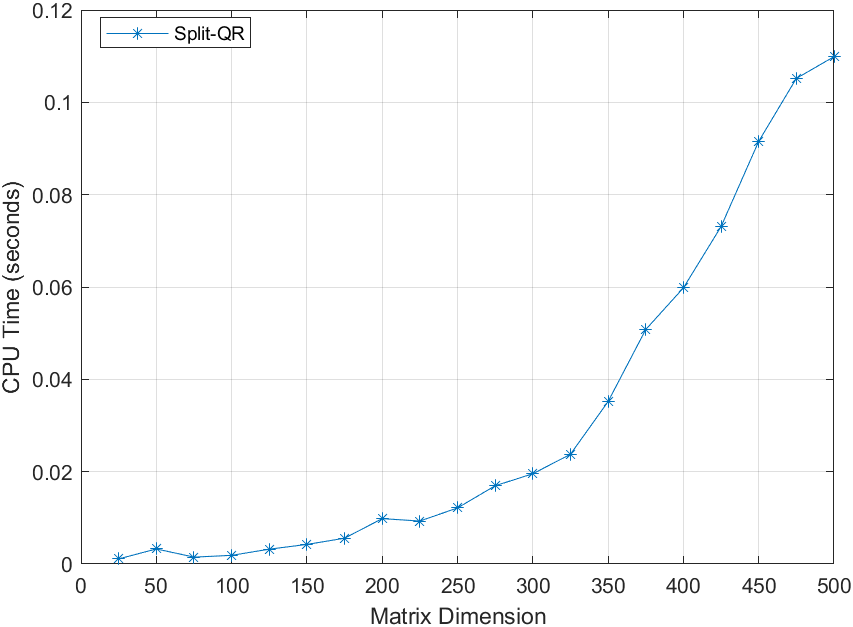
\includegraphics[width=\textwidth]{cpu times.png} % Replace with actual filename
       % \subcaption{(a)}
    \end{minipage}
    \hfill % Add space
    \begin{minipage}[b]{0.45\textwidth}
        \centering
        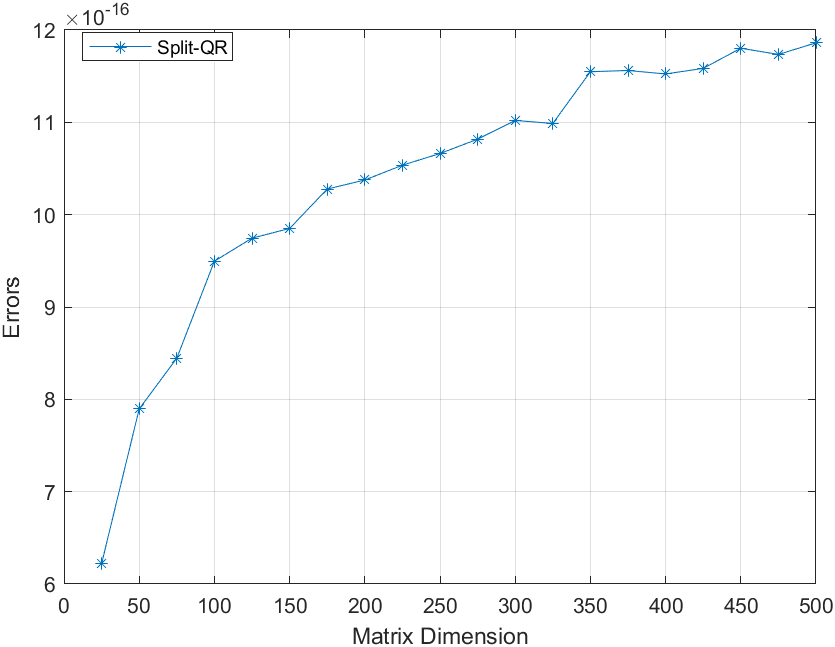
\includegraphics[width=\textwidth]{error.png} % Replace with actual filename
        % \subcaption{(b)}
    \end{minipage}
    % \captionsetup{font=footnotesize}
    \caption{ CPU Time and Error Analysis of the QR Algorithm for Split Quaternion Matrices }
     \label{fig:cpu times}
\end{figure}


Below, we will discuss the application of QR decomposition in solving matrix equation.
\begin{example}
Utilize the QR algorithm to solve the split quaternion matrix equation $AX = B$, where
\begin{align*}
A =
\begin{bmatrix}
-4 & -2 & -8 \\
-2 & -2 & -5 \\
7 & -3 & -9
\end{bmatrix} +
\begin{bmatrix}
-1 & -2 & 4 \\
-5 & -8 & -5 \\
-4 & 0 & 6
\end{bmatrix} i 
+ 
\begin{bmatrix}
-9 & -6 & -8 \\
-2 & -10 & -5 \\
-10 & -7 & -7
\end{bmatrix} j +
\begin{bmatrix}
-8 & 9 & -3 \\
2 & -6 & 0 \\
8 & 0 & -5
\end{bmatrix} k,
\end{align*}

\begin{align*}
B =
\begin{bmatrix}
-9 & -10 & 10 \\
-1 & 10 & 6 \\
-7 & -1 & -10
\end{bmatrix} +
\begin{bmatrix}
4 & 1 & -6 \\
4 & -6 & -3 \\
3 & 6 & 8
\end{bmatrix} i 
+
\begin{bmatrix}
7 & 2 & 2 \\
-2 & 9 & -4 \\
-4 & 9 & 7
\end{bmatrix} j +
\begin{bmatrix}
-1 & 1 & -3 \\
8 & 5 & -7 \\
-10 & -7 & -4
\end{bmatrix} k.
\end{align*}
\end{example}  
First, perform QR decomposition on $A$ to obtain $Q$ and $R:$
% \setlength{\jot}{5pt}
% \setlength{\arraycolsep}{1pt}
% {\footnotesize
\begin{align*}
Q =
& \begin{bmatrix}
-0.514 & -0.047 & -0.344 \\
-0.126 & -0.411 & -0.041 \\
-0.436 & -0.429 & -0.099
\end{bmatrix} +
\begin{bmatrix}
-0.363 & 0.479 & 0.122 \\
0.077 & -0.458 & -0.100 \\
0.383 & -0.194 & 0.138
\end{bmatrix} i \\
+ 
& \begin{bmatrix}
-0.236 & -0.062 & -0.155 \\
-0.105 & 0.031 & 0.403 \\
0.262 & 0.178 & -0.296
\end{bmatrix} j +
\begin{bmatrix}
-0.157 & 0.171 & 0.319 \\
-0.250 & -0.133 & 0.577 \\
-0.152 & 0.291 & -0.343
\end{bmatrix} k,\\
R =
& \begin{bmatrix}
-3.041 & 3.419 & 10.927 \\
0 & 6.061 & 6.456 \\
0 & 0 & 7.714
\end{bmatrix} +
\begin{bmatrix}
-1.443 & 8.617 & 1.053 \\
0 & 1.847 & -2.947 \\
0 & 0 & -5.025
\end{bmatrix} i \\
+ 
& \begin{bmatrix}
20.361 & 5.876 & 6.740 \\
0 & 14.697 & 6.795 \\
0 & 0 & 0.815
\end{bmatrix} j +
\begin{bmatrix}
1.443 & -2.642 & 6.596 \\
0 & -1.847 & -1.528 \\
0 & 0 & 5.025
\end{bmatrix} k.
\end{align*}
% }
Thus, the equation can be rewritten as
\begin{equation}
    QRX = B.\label{eq:example1}
\end{equation}
Since \(Q\) is a unitary matrix, \iffalse  \(Q^{-1} = Q^H\),\fi
multiplying both sides of \eqref{eq:example1} by \(Q^H\) from the left yields \(RX = Q^HB\triangleq\hat{B}\),
where
\begin{align*}
\hat{B} =
& \begin{bmatrix}
4.981 & 6.383 & 8.076 \\
-2.019 & -1.922 & -1.440 \\
11.356 & 10.929 & -9.652
\end{bmatrix} +
\begin{bmatrix}
-1.144 & -7.725 & 6.206 \\
1.152 & 11.947 & -2.239 \\
-3.761 & 0.482 & -0.749
\end{bmatrix} i \\+
& \begin{bmatrix}
-6.136 & -7.249 & -9.693 \\
0.310 & -4.646 & 0.574 \\
1.391 & -2.620 & -3.994
\end{bmatrix} j +
\begin{bmatrix}
11.385 & -4.261 & -2.859 \\
-7.851 & 1.655 & -0.404 \\
-0.653 & 6.826 & 12.841
\end{bmatrix} k.
\end{align*}
Note that \(R\) is an upper triangular matrix, thus  \(RX = Q^HB\triangleq\hat{B}\)  can be solved using back substitution:
 \begin{align*}
X =
& \begin{bmatrix}
-1.082 & -0.797 & 1.407 \\
-0.316 & -0.028 & 0.749 \\
1.846 & 0.845 & -2.243
\end{bmatrix} +
\begin{bmatrix}
-1.116 & -0.337 & 0.999 \\
-0.423 & -0.961 & 1.907 \\
0.349 & 1.315 & -0.403
\end{bmatrix} i \\+
& \begin{bmatrix}
-0.456 & -0.123 & 1.793 \\
-1.222 & -0.449 & 1.810 \\
0.402 & -1.119 & -1.423
\end{bmatrix} j +
\begin{bmatrix}
0.944 & 0.982 & -1.597 \\
0.059 & -0.514 & 0.229 \\
-0.989 & -0.256 & 2.156
\end{bmatrix} k.
\end{align*}
And the relative error is $\frac{\|AX - B\|_F}{\|B\|_F} = 1.2412\times 10^{-15}$.

%-------------------- 参考文献 --------------------
\begin{thebibliography}{99}


\bibitem[Abłamowicz(2020)]{Abłamowicz2020} R. Abłamowicz, The Moore–Penrose inverse and singular value decomposition of split quaternions, Adv. Appl. Clifford Algebr. 33 (30) (2020)1–20.

\bibitem[Yasemin(2012)]{Yasemin2012} Y. Alag\"oz, K. Oral, and S. Y\"uce. "Split quaternion matrices." Miskolc Mathematical Notes 13.2 (2012) 223–232.


\bibitem[Cockle(1849)]{Cockle1849} J. Cockle, On systems of algebra involving more than one imaginary; and on equations of the fifth degree, Phil. Mag. 35 (1849) 434–437.

\bibitem[Gog(2022)]{Gog2022} M. Gogberashvili, (2+1)-Maxwell equations in split quaternions, Physics 4 (1) (2022) 329–363.

\bibitem[Hasebe(2010)]{Hasebe2010} K. Hasebe, Split quaternionic hopf map, quantum hall effect, and twistor theory, Phys. Rev. D 81 (4) (2010) 041702.

\bibitem[TJiang(2015)]{TJiang2015} T. Jiang, Z. Jiang, Z. Zhang, Algebraic techniques for diagonalization of a split quaternion matrix in split quaternion mechanics, J. Math. Phys. 56 (2015)083509.

\bibitem[Jiang(2018)]{Jiang2018}T. Jiang, Z. Zhang, Z. Jiang, Algebraic techniques for eigenvalues and eigenvectors of a split quaternion matrix in split quaternionic mechanics,Comput. Phys. Comm. 229 (2018) 1–7.

\bibitem[TJiang(2018)]{TJiang2018}T. Jiang, Z. Zhang, Z. Jiang, Algebraic techniques for Schrödinger equations in split quaternionic mechanics, Comput. Math. Appl. 75 (2018)2217–2222.

\bibitem[Le(2022)]{Le2022} E. Legrand, The geometry of dissipative mechanical systems: Using Jacobi manifolds and the split quaternion algebra, Delft University of
Technology, 2022.

\bibitem[Zhuo(2020)]{Zhuo2020} X. Liu and Z. He. On the split quaternion matrix equation $AX= B$. Banach Journal of Mathematical Analysis 14.1 (2020) 228-248.

\bibitem[Yang(2020)]{Yang2020} X. Liu and Y. Zhang. Least squares \(X = {X^{\eta}}^* \) solutions to split quaternion matrix equation \(AX{A^{\eta}}^*= B\). Mathematical Methods in the Applied Sciences 43.5 (2020) 2189-2201.

\bibitem[Xin(2019)]{Xin2019} X. Liu and Y. Zhang. Consistency of Split Quaternion Matrix Equations $AX^* - XB = CY + D$ and $X - AX^*B = CY + D$. Advances in Applied Clifford Algebras 29 (2019) 1-20.

\bibitem[Z(2022)]{Z2022} Z. Özdemir, A kinematic model of the Rytov’s law in the optical fiber via split quaternions: application to electromagnetic theory, Euro. Phys.J. Plus 137 (6) (2022) 1–13.

\bibitem[mma(2023)]{mma} İ. Öztürk, and M. Özdemir. On geometric interpretations of split quaternions. Mathematical Methods in the Applied Sciences 46.1 (2023) 408-422.

\bibitem[wang(2024)]{wang} K.W. Si, Q.W. Wang, L.M. Xie. A classical system of matrix equations over the split quaternion algebra. Advances in Applied Clifford Algebras 34.5 (2024) 51.

\bibitem[Wang(2023)]{Wang2023} G. Wang, T. Jiang, V.I. Vasil’ev, Z. Guo, An efficient method for Maxwell’s equations with a discrete double-curl operator in split quaternionic electromagnetics, Eur. Phys. J. Plus 341 (138) (2023) 1–6.

\bibitem[Wang(2021)]{Wang2021}G. Wang, T. Jiang, Z. Guo, D. Zhang, A complex structure-preserving algorithm for split quaternion matrix LDU decomposition in split quaternion mechanics, Calcolo 58 (34) (2021) 1–15.

\bibitem[Gang(2024)]{Gang2024}G. Wang, T. Jiang, V. Vasil’ev, and Z. Guo. On singular value decomposition for split quaternion matrices and applications in split quaternionic mechanics. Journal of Computational and Applied Mathematics 436 (2024) 115447.

\bibitem[yuan(2017)]{yuan}S.F. Yuan, Q.W. Wang, Y. Yu. On Hermitian solutions of the split quaternion matrix equation $AXB+CXD=E$. Advances in Applied Clifford Algebras 27 (2017) 3235-3252.

\bibitem[Zhang(2015)]{Zhang2015}Z. Zhang, Z. Jiang, T. Jiang, Algebraic methods for least squares problem in split quaternionic mechanics, Appl. Math. Comput. 269 (2015) 618–625.


\end{thebibliography}

\end{document}